\documentclass[10pt,conference]{IEEEtran}
\IEEEoverridecommandlockouts
% The preceding line is only needed to identify funding in the first footnote. If that is unneeded, please comment it out.
\usepackage{cite}
\usepackage{amsmath,amssymb,amsfonts}
\usepackage{algorithmic}
\usepackage{graphicx}
\usepackage{textcomp}
\usepackage{xcolor}
\usepackage{subfig}
\usepackage{listings}
\lstset{numbers=left,stepnumber=1,basicstyle=\footnotesize\ttfamily}
\def\BibTeX{{\rm B\kern-.05em{\sc i\kern-.025em b}\kern-.08em
T\kern-.1667em\lower.7ex\hbox{E}\kern-.125emX}}
\def\code#1{\texttt{#1}}
\begin{document}

\title{A Second Look at the Dynamics of the JavaScript Package Ecosystem\\}

\author{\IEEEauthorblockN{Kevin de Haan, Gregory Neagu, Frederic Sauve-Hoover, Abram Hindle}
  \IEEEauthorblockA{\textit{Department of Computing Science} \\
    \textit{University of Alberta}\\
    Edmonton, Canada\\
  Email: \{kdehaan,neagu,rsauveho,abram.hindle\}@ualberta.ca}
}

\maketitle

% Footnote should maybe be a full source, or just one link
\begin{abstract}
  In recent years, the tools and packages most commonly involved with JavaScript development have evolved rapidly.
  Newer packages such as Angular and React have experienced a marked increase in popularity among developers, while frameworks such as jQuery
  have begun to phase out.\footnote{\label{adoption}https://insights.stackoverflow.com/survey/2016\#technology-most-popular-technologies, 
  https://insights.stackoverflow.com/survey/2017\#technology-\_-frameworks-libraries-and-other-technologies, 
  https://insights.stackoverflow.com/survey/2018\#technology-\_-frameworks-libraries-and-tools}
  For this reason we take a second look at a 2016 paper by Wittern, Suter and Rajagopalan \cite{Wittern:2016} 
  to see what aspects of the JavaScript package ecosystem have changed, and if previously observed trends have remained constant.
  In the original paper the authors use the \emph{node package manager} (\code{npm}) to gain 
  insight into the JavaScript ecosystem as a whole, and data from projects publicly hosted on 
  \code{GitHub} to observe an alternative measure of popularity. We adhere to the same methods of analysis, 
  and extend the data to capture more recent information up to April 1\textsuperscript{st} 2019.
  Ultimately, this second look aims to discover if recent years have had any significant effects on 
  ecosystem-wide trends, and provide developers with further insight into how packages are used and evolve.
\end{abstract}


\begin{IEEEkeywords}
  JavaScript; Node.js; node package manager; software ecosystem analysis
\end{IEEEkeywords}


\section{Introduction}
Software ecosystems are environments that form as projects develop in parallel,
becoming interconnected as contexts and dependencies span companies and communities \cite{LUNGU2010264}. 
Research on these systems has increased rapidly in the recent past \cite{Manikas:2017}, investigating
their characteristics and behaviour as they develop \cite{Manikas:2013}. Understanding how software
ecosystems evolve is important from both a software as well as a business standpoint\cite{Messerschmitt},
and is valuable for informing developers how technologies are used over time \cite{Serebrenik:2015}. 
An understanding of software ecosystems can inform decisions on when to adopt frameworks and how long
to support them, as well as provide insight into how changes to software propagate throughout the community \cite{Wittern:2016}.
Additionally, determining the characteristics of software ecosystems 
can help clarify why some frameworks flourish while others fail, and guide 
developers in the creation of new tools\cite{Serebrenik:2015}. Furthermore, 
because software projects are overwhelmingly a collaborative effort, a complete
understanding of a single project often requires knowledge of the ecosystem supporting it\cite{Blincoe:2015}.


This paper is a replication of \emph{A Look at the Dynamics of the JavaScript Package Ecosystem}\cite{Wittern:2016} 
that performs extensive analysis of the \emph{node package manager} (\code{npm}) ecosystem. 
\code{npm} provides a set of open source tools that allow developers to 
describe packages for \code{Node.js}, an asynchronous JavaScript runtime environment 
designed for network applications\footnote{https://nodejs.org/en/about/}.
The services provided by \code{npm} include a command line interface for maintaining 
\code{package.json} files, the primary method to describe package metadata such as the name,
description, version, and dependencies of a given package. \code{npm} also allows 
developers to publish their packages to a public registry, permitting anyone 
to download and use their software. Packages hosted on \code{npm} will often depend on other \code{npm}
packages, forming an elaborate JavaScript package ecosystem.
Since the publishing of the original paper, the usage and scale of \code{npm} has only grown,
and now hosts more than three times as many packages (over 750,000 as of April 1\textsuperscript{st} 2019) 
and handles over ten times as many weekly package downloads (now over ten billion per week).
Additionally, the major frameworks used in JavaScript development have undergone a 
rapid transformation as packages such as Angular and React are adopted\footnotemark[\ref{adoption}].
The core contributions we make are as follows:
\begin{itemize}
  \item We replicate and verify the results found in the original paper for the 
    window of October 1\textsuperscript{st} 2010 to September 1\textsuperscript{st} 2015.
  \item We extend the analysis to the time period of September 2\textsuperscript{nd} 
    2015 to April 1\textsuperscript{st} 2019, and evaluate whether patterns and trends 
    noted in the original paper are still observable.
  \item We investigate whether the continued evolution of the JavaScript package 
    ecosystem has affected the relationships between various measures of package popularity.
  % \item We determine if the ongoing maturation of the \code{npm} ecosystem has 
  %   resulted in tangible changes to version numbering or adoption practices.
\end{itemize}


\section{Data Collection}
% CHECK IF THE NUMBERS ARE RIGHT
The window of data analyzed within this paper is October 1\textsuperscript{st} 2010 (as in the original paper) to April 1\textsuperscript{st} 2019.
We collected from three publicly available data sets. Two of these, the \code{npm} registry and the \code{GitHub} repository platform, are from the same source as in the original paper.
To find repositories relying on \code{npm}, we used the Google BigQuery \code{github\_repos} data set, updated weekly\footnote{https://github.com/fhoffa/analyzing\_github/}.
By using this set we are able to analyze \code{GitHub} data without being constrained to the currently available window provided by the GHTorrent project\cite{Gousi13}.
The final data set encompasses 797,940 packages and 40,000 applications.

\subsection{Package Metadata} \label{PackageMetadata}

\begin{lstlisting}[caption={A mock \code{npm} package.json. Some fields omitted for brevity.},captionpos=b,
  label=samplePkg, frame=single, firstline=1]
{
  "name": "Lorem Ipsum",
  "version": "0.9.3",
  "maintainers": [
      {"name": "Dolor Sit",
      "email": "dolorsit@amet.org"}
  ],
  "repository": {
      "type": "git",
      "url": "https://github.com/lor/em"
  },
  "main" : "loremipsum.js",
  "keywords": ["Web", "REST"],
  "dependencies": {
      "Adipiscing": "~1.7.0",
      "Elit": "5.1.x"
  },
  "devDependencies": {
      "Sed": "0.9.0",
      "Do": ">=1.3.5 <4.0.0" 
  }
}
\end{lstlisting}

\begin{lstlisting}[caption={A mock simplified \code{npm} metadata file.},captionpos=b,
  label=sampleSimpleMetadata, frame=single, firstline=1]
{
  "name": "Lorem Ipsum",
  "versions": {
    "1.0.4": {
      "dependencies": {
        "Adipiscing": "~1.7.0",
        "Elit": "5.1.x"
      },
      "devDependencies": {
        "Sed": "0.9.0",
        "Do": ">=1.3.5 <4.0.0"
      }
    },
    "1.0.5": {
      "dependencies": {
        "Adipiscing": "~1.7.0",
      },
      "devDependencies": {
        "Do": ">=1.3.5 <4.0.0"
      }
    },
    "time": {
      "1.0.4": "2017-09-25T06:39:20.596Z",
      "1.0.5": "2018-05-22T08:35:40.227Z",
      "created": "2015-05-18T03:52:55.192Z"
    }
  }
}
\end{lstlisting}

Metadata for every package is available on the \code{npm}
registry\footnote{https://registry.npmjs.org/packageName}. 
This metadata is a \code{JSON} file containing info 
on licensing, documentation links, and maintainers, as well as
a log of each version of the package since its creation, which 
for our purposes is the most crucial element.
The version data is labelled using semantic 
versioning \cite{preston-werner} and includes a time field containing 
the timestamp of creation for each version. Each version in the version 
field contains various version specific information such as authors, 
maintainers, the license used, bugs, and a list of dependencies for that specific
version.

We obtained the list of all \code{npm} package names from 
the \code{npm} registry \code{skimdb}\footnote{https://skimdb.npmjs.com/registry/\_all\_docs}. Using these names,
we then downloaded the metadata for each of the 797,940 packages hosted by the
\code{npm} registry and then converted this metadata into a somewhat simplified form 
with just version and dependency information, as seen
in Listing \ref{sampleSimpleMetadata}. There are two kinds of dependencies in the metadata
files: runtime dependencies and \code{devDependencies} used in testing and development.

% We gathered information on download counts for \code{npm} packages from the
% \code{npm} API\footnote{https://api.npmjs.org/downloads/range/2010-01-01:2019-04-01/packageName} 
% however we found that the npm.js API seems to no longer have any data on download counts before October 1 2017, and so were unable to collect
% historic download counts for \code{npm} as a whole or any specific packages.\\

\subsection{Applications using \code{npm} Packages}

To collect our data for package usage in public projects, 
we turned to the Google BigQuery \code{github\_repos} data 
set\footnote{https://bigquery.cloud.google.com/dataset/bigquery-public-dat:github\_repos}.
From this data, we skimmed all projects and pulled those 
written in JavaScript, resulting in an initial total of 9,017,221 
repositories. Simply being written in JavaScript is not enough to detect
\code{npm} usage, so to find repositories using \code{npm} packages
we looked for projects that contained a \code{package.json} 
file. After confirming that the formatting of the file matched the \code{npm}
standard, we are able to confidently say that any remaining packages are 
using \code{npm} packages. With this criteria, we then compiled a list 
of [100,000 for now] project 
repositories from GitHub, a volume that we felt is likely to be an 
appropriate representation of all such public projects.
Using the \code{GitHub} platform API and the list of valid repository names 
from before, we cloned the GitHub repository for each project. With
this, we were then able to determine the date and time of every 
commit of the project, as well as the list of included \code{npm} packages
at the time of commit, as listed in every historic version of 
\code{package.json}, providing us with the \code{npm} packages used by that repository
at any given time in the project's history. The results showed that on average a repository 
had 37.9 commits. Ultimately, of the 9,017,221 
public \code{GitHub} projects written in JavaScript and out of all of the repositories
using \code{npm} packages, we randomly selected 40,000 repositories as
a representative data set for the analysis.


\section{Ecosystem Evolution}

\begin{figure}
  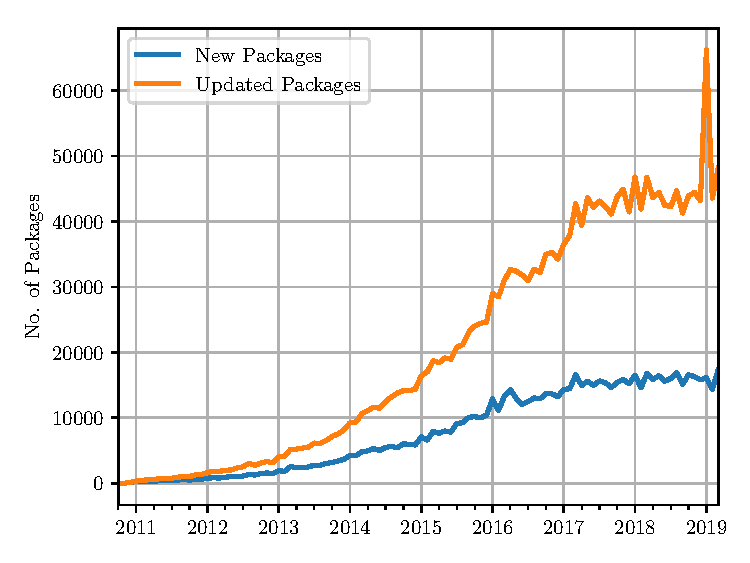
\includegraphics[width=0.5\textwidth]{figures/new_vs_updates_by_month.pdf}
  \caption{Packages updated and packages created per month. Multiple updates per month are
  only counted once.}
  \label{npmGrowth}
\end{figure}

Created in 2009, \code{npm} has grown
rapidly in popularity and scope over the last ten years, and 
as of the original paper showed no signs of slowing down \cite{Wittern:2016}.
We investigate the state of the \code{npm} ecosystem
since September 1\textsuperscript{st} 2015, and look for any signs of deterioration in 
the health of the ecosystem. Periods of stagnating growth would suggest
that developer interest is waning, while steady activity would 
indicate that the ecosystem as a whole is healthy and will continue to
evolve. To search for these potential indicators in the \code{npm} package environment,
we investigate the number of packages created and updated over time, as well
as system-wide trends of dependencies within packages. 
In Figure \ref{npmGrowth},
we can observe that while \code{npm} is still growing, the speed at which new packages
are created has slowed from an exponential to a linear rate. Packages added and updated 
per month have gone from 10,087 and 23,100 respectively in September 2015 to 17,354 and 48,140 respectively as of April 2019.
Some other things of note include an observable spike in package creation and updates around March 2016, the month 
when developer Azer Ko\c{c}ulu removed his 273 packages (including the popular package 
\code{left-pad}) from \code{npm} and in doing so affected some packages such as 
\code{babel} and \code{atom}, and therefore a significant fraction of \emph{all} 
\code{Node.js} projects\footnote{https://blog.npmjs.org/post/141577284765/kik-left-pad-and-npm}.
There is also a significant spike in package updates observed in the month of January 2019, caused 
by some source currently unknown to the authors.
[ADD CONCAVITY DATA]. 

\begin{figure}
  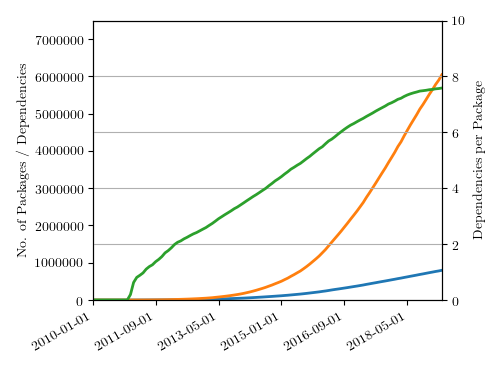
\includegraphics[width=1\linewidth]{figures/packages_vs_dependencies.png}
  \caption{Axis \code{y1} shows growth in number of \code{npm} packages (blue line), and the number of package dependencies (orange line) over time. 
  Axis \code{y2} shows the average number of dependencies per package (green line).}
  \label{packVSDependencies}
\end{figure}

Figure \ref{packVSDependencies} presents the total number of \code{npm} packages over time, 
as well as the total number of package dependencies. Additionally, we have plotted
the average number of dependencies per \code{npm} package. Curiously, though total dependencies
continues to grow faster than the creation of new packages, the number of dependencies 
for the average package appears to be plateauing. If this trend continues, it could suggest
that the \code{npm} ecosystem is reaching some sort of equilibrium with regards to the number
of package dependencies.

\begin{figure}
  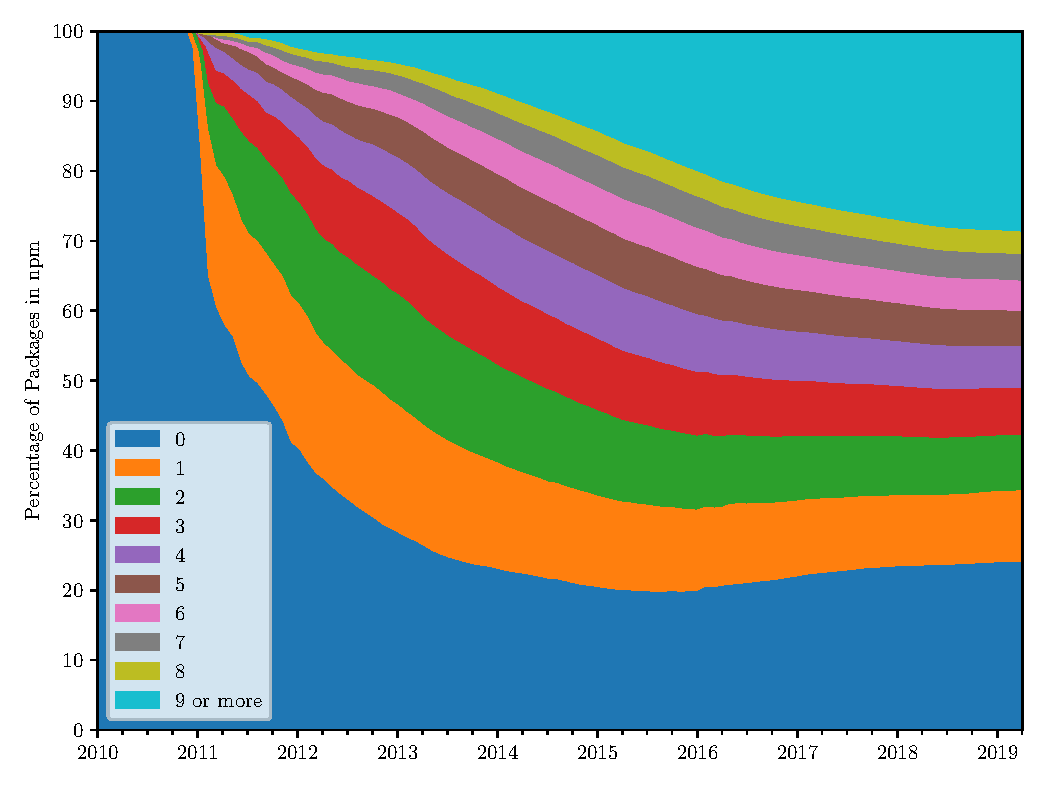
\includegraphics[width=0.5\textwidth]{figures/npm_deps_monthly_out_degree.pdf}
  \caption{\code{npm} packages by their number of dependencies on other packages.}
  \label{outDegree}
\end{figure}

To better visualize the status of inter-package dependencies, we constructed
a directed dependency graph using dependants as out-degrees and
dependencies as in-degrees. Based on this data, Figure \ref{outDegree}
displays the percentage of packages with various amounts of dependencies. 
This confirms some of our earlier suspicious: while the average number of dependencies 
of packages continues to increase, the percentage of packages with zero 
to three dependencies has actually increased since the end of the original paper's
reporting period \cite{Wittern:2016}. This supports the hypothesis that developer 
behaviour is changing, likely either as a deliberate effort by programmers seeking to avoid the perils of 
complicated dependency trees \cite{Kikas:2017}, or as a natural result of the ever-changing
ways in which JavaScript is used for project development. In particular, the number of packages with zero dependencies
has increased from 19.5\% in September 2015 to 23.8\% as of April 2019.

\begin{figure}
  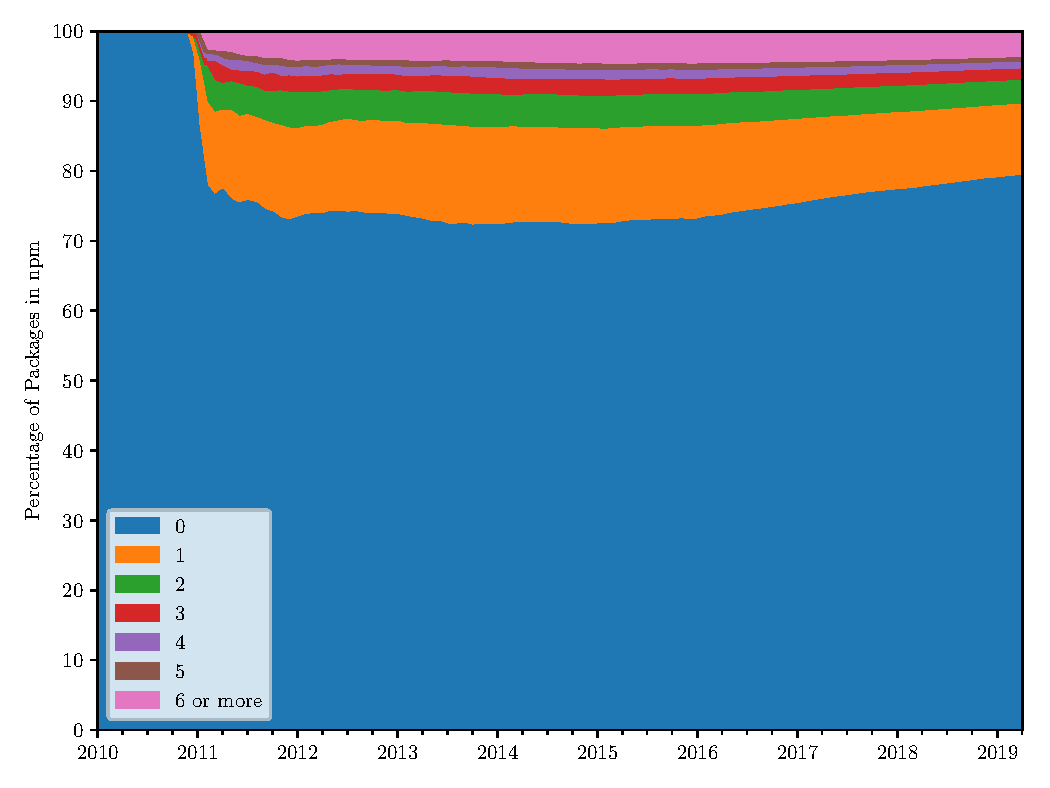
\includegraphics[width=0.5\textwidth]{figures/npm_deps_monthly_in_degree.pdf}
  \caption{\code{npm} packages by the number of other packages depending on them.}
  \label{inDegree}
\end{figure}

In addition to the number of external dependencies per package, 
we investigate how packages support dependants. The original paper 
discovered that the majority of in degrees are concentrated among a core 
minority of packages, with the majority of packages having no dependants,
a discovery that has also been observed in other software ecosystems such
as Linux and MySQL \cite{Myers:2003}. In our updated data, we discover 
that not only have these aspects held true, but the concentration of 
dependencies has actually increased. As of April 1\textsuperscript{st} 2019, 79.2\% of packages
had zero dependants, up from 72.8\% in September 2015. Meanwhile, only 3.2\% of packages
had 6 or more dependants, down from 3.8\% in September 2015. It is again interesting to note
that the current trend of increasing concentration appears to have begun shortly after the end of window in the original
paper.

In section \ref{popularity}, we revisit the popularity measures
investigated in the original paper \cite{Wittern:2016} to discover
changes in the relationships between package rankings
both inside and outside of the \code{npm} ecosystem,
gaining insight into the dynamics of \code{npm} package popularity.

\textbf{Takeaways.} We find that while the \code{npm} ecosystem
continues to grow, the rate of growth is no longer superlinear, 
a possible sign of the ecosystem beginning to reach some form of maturity \cite{Alves:2011}.
In the relationships between packages, we find that though the average number
of dependencies continues to grow, there has been a recent decline in the
rate of this growth. Accordingly, we have found that the number of packages with
zero dependencies has increased from 28.7\% in September 2015 to [DATA REQUIRED]\%
as of April 2019. The percentage of packages that are depended on has
also declined, albeit still exhibiting a power law relationship as observed
in prior software ecosystem research \cite{Wittern:2016, Myers:2003, Louridas:2008}.


\section{Package Popularity}\label{popularity}

As per the original paper we analyzed popularity of \code{npm} packages using three major measures \cite{Wittern:2016}:
\begin{enumerate}
  \item The \textbf{\code{npm} rank} is calculated using the PageRank\cite{brin1998anatomy} of an \code{npm} package within a dependency graph that we built using the
    package metadata as described in Section \ref{PackageMetadata}. PageRank is calculated for every package using a damping factor of 0.85 
    and stopping iterations once the cumulative change in values of vertices went below $10^{-6}$. We then order all packages by their PageRank to determine the
    \code{npm} rank, an relative ranking of package popularity with 1 being the most popular.
  \item The \textbf{download rank} of a package is based on the the gross volume of package downloads from the \code{npm}
    registry, then ordered relatively with 1 being the most downloaded.
  \item \textbf{\code{GitHub} rank} is a measure of the popularity of a package among public \code{GitHub} projects.
    This rank is created from a list of \code{npm} dependency occurrences found in \code{package.json} files, with rank 1
    meaning that the package was the most common dependency among analyzed \code{GitHub} repositories.  
\end{enumerate}


\subsection{Relationships between Measures}
[NEEDS MORE DATA]

\subsection{Distinct Package Types}
[NEEDS MORE DATA]

\subsection{Popularity Over Time}

With the differences and changes in the relationships between
popularity measures explored, we can now focus on \code{npm}
rankings in particular, as it is most representative of the 
importance of a package to the \code{npm} ecosystem as a whole.
To obtain \code{npm} ranks over time, we first begin with the
complete dependency graph as of April 2019. We then examine
the date references on the edges of the graph to produce \code{PageRanks}
for each and every package on a monthly basis for the period of October 2010
to April 2019. From the list of \code{PageRanks} in each month, we then
produce the relative rank for every package present in the \code{npm}
ecosystem at that time. 

\subsubsection{Identifying Top Packages}

\begin{figure}
  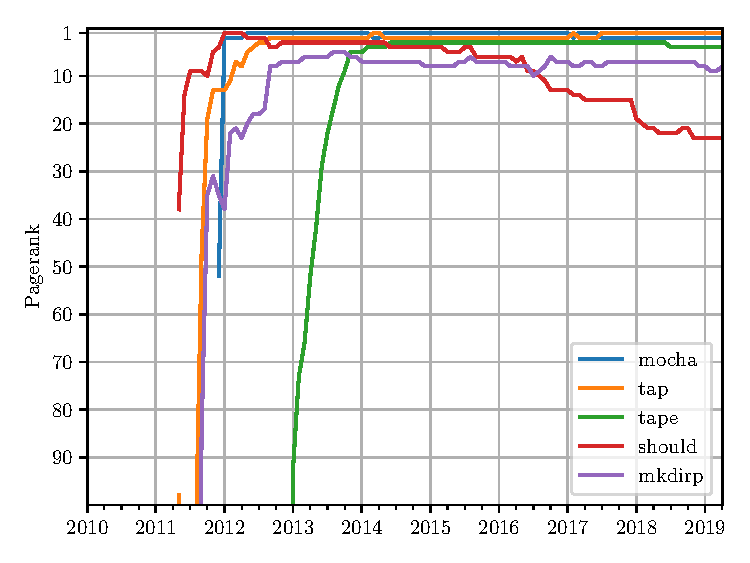
\includegraphics[width=0.5\textwidth]{figures/geo_mean_highest_pagerank.pdf}
  \caption{\code{npm} rank (PageRank) of the five packages with the lowest overall geometric mean}
  \label{topFive}
\end{figure}

One of the most obvious things to investigate is which packages
have historically performed best throughout the entirety of 
\code{npm}'s existence. To determine overall package popularity,
we use the geometric mean \code{npm} rank of a package over the full 
window of analysis, and order them from lowest to highest (i.e,
highly ranked to lowly ranked). Geometric mean is used in this instance
instead of arithmetic mean in order to limit the effect of outliers \cite{Wittern:2016}.
With popularity calculated in this manner, Figure \ref{topFive} presents 
the top five \code{npm} packages of all time.

The first thing to notice about these five packages is that the rankings
have changed since the time of the original paper. Gone are the packages
\code{uglify-js} and \code{coffee-script}, and newcomers \code{tape} and \code{mkdirp}
have appeared. Additionally, though the package \code{should} remains on the list,
it has fallen from the \#2 to the \#4 position. 

Four of the five current champions are testing utilities---\code{mkdirp} is the sole exception, instead providing the ability to dynamically
create directories from within \code{node.js}. Curiously, the testing packages
are essentially all direct competitors of one another, providing a powerful 
demonstration of both the widespread importance of testing utilities as well as
the ability for the \code{npm} software ecosystem to support multiple core packages with
similar yet distinct functionality.

\begin{figure*}
  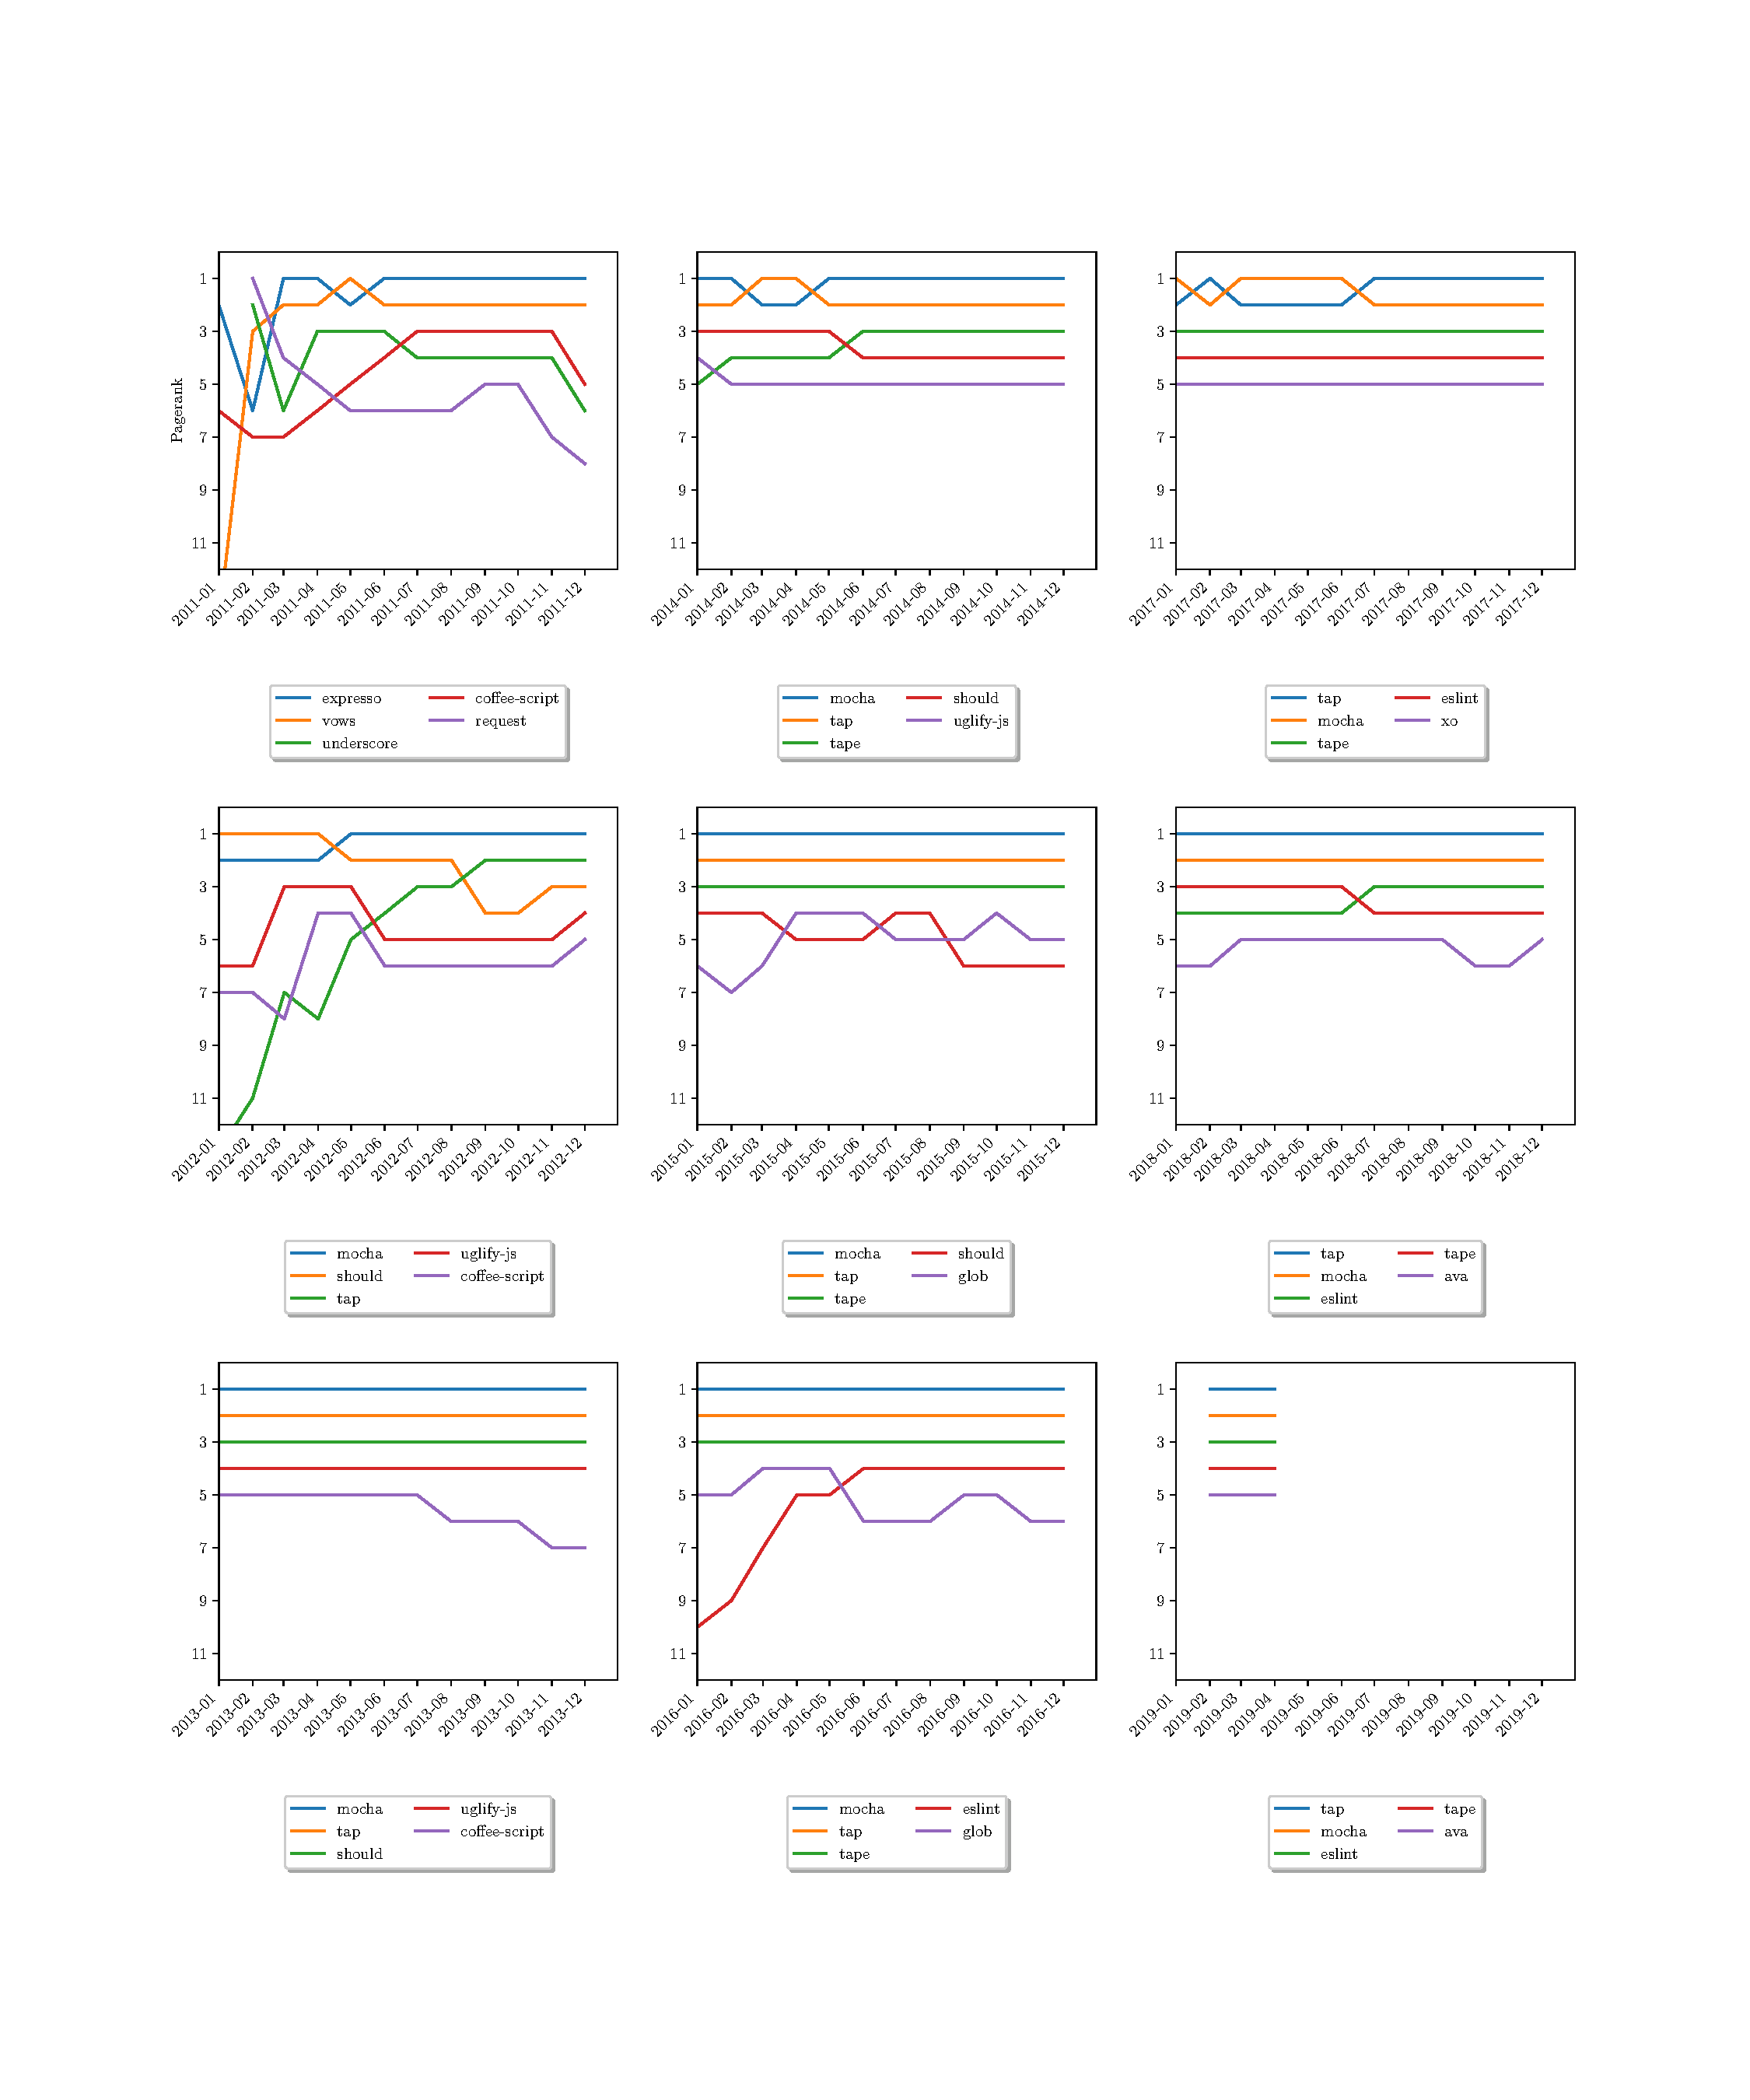
\includegraphics[width=1\textwidth]{figures/highest_ranked.pdf}
  \caption{\code{npm} rank (PageRank) of the five packages each year with the lowest geometric}
  \label{ranksByYear}
\end{figure*}

While these packages represent the most consistently popular
members of \code{npm}, we also evaluate the most popular packages
on a yearly basis. Figure \ref{ranksByYear} presents the top five packages
for each individual year from 2011 to 2019. As noted in the original paper,
the top packages per year are relatively stable from 2013 on \cite{Wittern:2016}.
One notable exception to this rule is the 2016 rise in popularity of \code{eslint},
a tool for improving the quality of \code{JavaScript} code\footnote{https://www.npmjs.com/package/eslint}.


\subsubsection{Popular Package Dynamics}

To better understand the evolution of package popularity,
we investigate the dynamics of the top rankings over time.
While figure \ref{ranksByYear} demonstrate that package popularity
appears to be relatively stable, we can examine the number of packages
entering (and therefore exiting) the top \code{n} packages per year in
order to obtain a better view of the ecosystem as a whole.
Table \ref{numEnteringTop} depicts the amount of newcomers to the top
\code{npm} ranks each year, further supporting the observation that
core \code{npm} package popularity is becoming more stable as the 
ecosystem matures.

\begin{table}
  \centering
  % TODO NOTE THAT THIS HAS LOWER NUMBERS THAN THE ORIGINAL PAPER DUE TO MONTHLY PAGERANKS
  \begin{tabular}{c|c|c|c}
    Year & Top 10 & Top 100 & Top 250 \\
    \hline
    2010 & 13 & 103 & 253\\
    2011 & 25 & 297 & 701\\
    2012 & 6 & 46 & 136\\
    2013 & 3 & 38 & 114\\
    2014 & 1 & 40 & 96\\
    2015 & 4 & 38 & 86\\
    2016 & 4 & 29 & 62\\
    2017 & 0 & 12 & 48\\
    2018 & 0 & 15 & 31\\
    2019 & 0 & 4 & 12\\
  \end{tabular}
  \caption{Number of packages entering top \code{npm} ranks for the first time}
  \label{numEnteringTop}
\end{table}


\subsubsection{Comparing the Popularity of Similar Packages}

\begin{figure}
  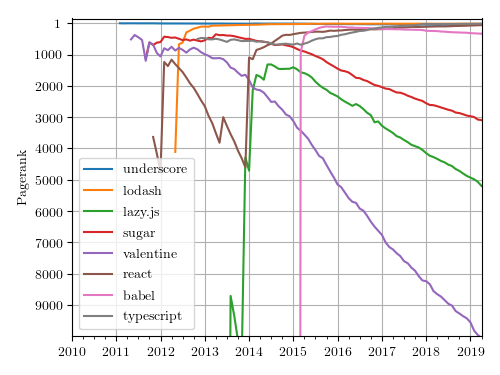
\includegraphics[width=0.5\textwidth]{figures/select_packages.png}
  \caption{\code{npm} rank (PageRank) over time of selected utility packages}
  \label{selectPackages}
\end{figure}

One of the significant benefits of being able to determine
\code{npm} ranks over time is that it allows for the comparison
of similar packages against each other at an objective level.
Figure \ref{selectPackages} shows the npm ranks of selected 
utility packages, as chosen in the original paper \cite{Wittern:2016}.
One of these packages, \code{underscore}, is among the oldest \code{npm} 
utility packages, and the rest have been selected for being
typical alternatives to the \code{underscore} package. Some of these packages,
such as \code{lodash}, are directly or indirectly results of forks from the
\code{underscore} repository. While \code{lodash} has kept up and even surpassed
\code{underscore} in popularity, the majority of newer alternatives are unable
to consistently compete. Calculating ranks for similar groups of packages such as
this allow us to isolate notable, successful packages across the entire span of
the ecosystem's history, as well as evaluate the persistence of the most popular
core packages over time. In the example group of packages presented in Figure \ref{selectPackages},
we can observe that the package established early in the ecosystem's life-cycle
is well-positioned to maintain a significant level of popularity, while the majority of
other packages tend to eventually decline unless they provide something exceptional,
such as \code{lodash} providing API compatibility with \code{underscore}\footnote{https://lodash.com/}.

\textbf{Takeaways.} Using \code{npm} ranks, we are able to identify successful packages 
at any point in the life-cycle of the ecosystem. We can also use these
ranks to obtain a measure of package popularity stability over time. In 
the \code{npm} ecosystem, the amount of change in the highest ranked packages
has decreased significantly since the inception of the service, with many
more recent utilities falling out of favour relative to the oldest and most
historically successful equivalents. However, there are still some relatively newer 
packages such as \code{lodash} that have managed to compete with the oldest core packages
such as \code{underscore}.
% \section{Version Numbering and Package Adoption}
% [NEEDS MORE DATA]

% \subsection{Attribution of Version Numbers}
% [NEEDS MORE DATA

% \subsection{Adoption by Version Number}
% [NEEDS MORE DATA]

\section{Related Work}

Related research can be generally described as one of two types
of work: meta-analyses of the behaviour and importance
of software ecosystems, and empirical investigations into the
specifics of a particular ecosystem. Some topics 
for meta-analyses include ecosystem visualization \cite{LUNGU2010264},
ecosystem maturity \cite{Alves:2011}, quality metric aggregation \cite{Mordal:2013},
and literature reviews \cite{Manikas:2013, Manikas:2017}. Specific ecosystem analysis include works such as this
paper as well as the original research by Wittern, Suter and Rajagopalan \cite{Wittern:2016} on \code{npm}.
Others have performed evaluations of specific ecosystems such as Raemaekers et al. \cite{Raemaekers:2013},
who present a dataset with basic metrics, dependencies and changes within the popular 
Java-based Maven ecosystem. Another work investigates the
result of changing project interdependencies in Apache \cite{Bavota:2013}, 
and still others evaluate evolution over time in ecosystems like
Gentoo \cite{Bloemen:2014}, Ruby, \cite{Kabbedijk:2011}, and R \cite{Plakidas:2017}.
Some works have looked empirically at the results of changing versions
within software ecosystems (including \code{npm}), finding that
developers often encounter difficulties when attempting to avoid
breaking dependencies \cite{Bogart:2015}.

Finally, \code{npm} has been investigated informally. In
the \code{pagerank} package, web-based \code{PageRanks} are used to evaluate
package popularity\footnote{https://www.npmjs.com/package/pagerank}.
The project code{npm-by-the-numbers} also provides various statistics
about the state of \code{npm}, but is significantly out of date and 
in contrast to this work does not provide an evaluation of the ecosystem over time
or give any insight into application usage\footnote{https://github.com/ashleygwilliams/npm-by-the-numbers}.


\section{Conclusion}

In this paper, we take a second look at the \code{npm} ecosystem,
replicating and extending the results of previous research by 
Wittern, Suter and Rajagopalan \cite{Wittern:2016}. Though
we observe that the growth of \code{npm} has slowed down, the ecosystem
continues to thrive, demonstrating signs of maturity rather than decline.

Contrary to the trend observed in the original paper, there appears to be
some effort to reduce the number of inter-package dependencies, and therefore the risks
associated with complex dependency trees. The core set of packages upon which
multiple other projects rely on has remained relatively constant in size, and
demonstrates a trend towards even further concentration. Accordingly, the set of packages
most depended on in the \code{npm} ecosystem is also trending towards stability, with
fewer and fewer packages entering the top ranks each year. 

Our results regarding relationships between popularity metrics support the discoveries of the
original paper, further reinforcing the theory that packages can be generally divided into the categories
of end user and core utility packages, and improving our understanding of how package popularity evolves.
Ultimately, our second evaluation of the \code{JavaScript} package environment can help developers evaluate
the state of the \code{npm} ecosystem, and continue to make informed decisions when selecting frameworks
to use in their applications.


\begin{thebibliography}{10}

  \bibitem{Alves:2011}
  Salviano~C.F Alves~A.M., Pessoa~M.
  \newblock {\em Towards a Systemic Maturity Model for Public Software
    Ecosystems}, volume 155.
  \newblock Springer, Berlin, Heidelberg, 2011.
  
  \bibitem{Bavota:2013}
  Gabriele Bavota, Gerardo Canfora, Massimiliano~Di Penta, Rocco Oliveto, and
    Sebastiano Panichella.
  \newblock The evolution of project inter-dependencies in a software ecosystem:
    The case of apache.
  \newblock In {\em Proceedings of the 2013 IEEE International Conference on
    Software Maintenance}, ICSM '13, pages 280--289, Washington, DC, USA, 2013.
    IEEE Computer Society.
  
  \bibitem{Blincoe:2015}
  Kelly Blincoe, Francis Harrison, and Daniela Damian.
  \newblock Ecosystems in github and a method for ecosystem identification using
    reference coupling.
  \newblock In {\em Proceedings of the 12th Working Conference on Mining Software
    Repositories}, MSR '15, pages 202--207, Piscataway, NJ, USA, 2015. IEEE
    Press.
  
  \bibitem{Bloemen:2014}
  Remco Bloemen, Chintan Amrit, Stefan Kuhlmann, and Gonzalo Ordonez-Matamoros.
  \newblock Gentoo package dependencies over time.
  \newblock pages 404--407, 05 2014.
  
  \bibitem{Bogart:2015}
  Christopher Bogart, Christian K{\"a}stner, and James Herbsleb.
  \newblock When it breaks, it breaks: How ecosystem developers reason about the
    stability of dependencies.
  \newblock In {\em Proceedings of the ASE Workshop on Software Support for
    Collaborative and Global Software Engineering (SCGSE)}, pages 86--89, 11
    2015.
  
  \bibitem{brin1998anatomy}
  Sergey Brin and Lawrence Page.
  \newblock The anatomy of a large-scale hypertextual web search engine.
  \newblock {\em Computer networks and ISDN systems}, 30(1-7):107--117, 1998.
  
  \bibitem{DBLP:Decan:2018}
  Alexandre Decan, Tom Mens, and Philippe Grosjean.
  \newblock An empirical comparison of dependency network evolution in seven
    software packaging ecosystems.
  \newblock {\em CoRR}, abs/1710.04936, 2017.
  
  \bibitem{Gousi13}
  Georgios Gousios.
  \newblock The ghtorrent dataset and tool suite.
  \newblock In {\em Proceedings of the 10th Working Conference on Mining Software
    Repositories}, MSR '13, pages 233--236, Piscataway, NJ, USA, 2013. IEEE
    Press.
  
  \bibitem{Kabbedijk:2011}
  Jaap Kabbedijk and Slinger Jansen.
  \newblock Steering insight: An exploration of the ruby software ecosystem.
  \newblock volume~80, pages 44--55, 06 2011.
  
  \bibitem{Kikas:2017}
  Riivo Kikas, Georgios Gousios, Marlon Dumas, and Dietmar Pfahl.
  \newblock Structure and evolution of package dependency networks.
  \newblock In {\em Proceedings of the 14th International Conference on Mining
    Software Repositories}, MSR '17, pages 102--112, Piscataway, NJ, USA, 2017.
    IEEE Press.
  
  \bibitem{Louridas:2008}
  Panagiotis Louridas, Diomidis Spinellis, and Vasileios Vlachos.
  \newblock Power laws in software.
  \newblock {\em ACM Trans. Softw. Eng. Methodol.}, 18(1):2:1--2:26, October
    2008.
  
  \bibitem{LUNGU2010264}
  Mircea Lungu, Michele Lanza, Tudor Gîrba, and Romain Robbes.
  \newblock The small project observatory: Visualizing software ecosystems.
  \newblock {\em Science of Computer Programming}, 75(4):264 -- 275, 2010.
  \newblock Experimental Software and Toolkits (EST 3): A special issue of the
    Workshop on Academic Software Development Tools and Techniques (WASDeTT
    2008).
  
  \bibitem{Manikas:2013}
  Konstantinos Manikas and Klaus~Marius Hansen.
  \newblock Software ecosystems - a systematic literature review.
  \newblock {\em J. Syst. Softw.}, 86(5):1294--1306, May 2013.
  
  \bibitem{Messerschmitt}
  David Messerschmitt and Clemens Szyperski.
  \newblock {\em Software Ecosystem: Understanding an Indispensable Technology
    and Industry}.
  \newblock 01 2003.
  
  \bibitem{Mordal:2013}
  Karine Mordal-Manet, Nicolas Anquetil, Jannik Laval, Alexander Serebrenik,
    Bogdan Vasilescu, and Stéphane Ducasse.
  \newblock Software quality metrics aggregation in industry.
  \newblock {\em Journal of Software: Evolution and Process}, 25:1117--1135, 10
    2013.
  
  \bibitem{Myers:2003}
  Christopher~R. Myers.
  \newblock Software systems as complex networks: Structure, function, and
    evolvability of software collaboration graphs.
  \newblock {\em Phys. Rev. E}, 68:046116, Oct 2003.
  
  \bibitem{DBLP:PanoGA16}
  Amantia Pano, Daniel Graziotin, and Pekka Abrahamsson.
  \newblock What leads developers towards the choice of a javascript framework?
  \newblock {\em CoRR}, abs/1605.04303, 2016.
  
  \bibitem{Plakidas:2017}
  Konstantinos Plakidas, Daniel Schall, and Uwe Zdun.
  \newblock Evolution of the r software ecosystem.
  \newblock {\em J. Syst. Softw.}, 132(C):119--146, October 2017.
  
  \bibitem{preston-werner}
  Tom Preston-Werner.
  \newblock Semantic versioning 2.0.0.
  
  \bibitem{Raemaekers:2013}
  Steven Raemaekers, Arie van Deursen, and Joost Visser.
  \newblock The maven repository dataset of metrics, changes, and dependencies.
  \newblock pages 221--224, 05 2013.
  
  \bibitem{Manikas:2017}
  M.~{Seppänen}, S.~{Hyrynsalmi}, K.~{Manikas}, and A.~{Suominen}.
  \newblock Yet another ecosystem literature review: 10+1 research communities.
  \newblock In {\em 2017 IEEE European Technology and Engineering Management
    Summit (E-TEMS)}, pages 1--8, Oct 2017.
  
  \bibitem{Serebrenik:2015}
  Alexander Serebrenik and Tom Mens.
  \newblock Challenges in software ecosystems research.
  \newblock In {\em Proceedings of the 2015 European Conference on Software
    Architecture Workshops}, ECSAW '15, pages 40:1--40:6, New York, NY, USA,
    2015. ACM.
  
  \bibitem{Wittern:2016}
  Erik Wittern, Philippe Suter, and Shriram Rajagopalan.
  \newblock A look at the dynamics of the javascript package ecosystem.
  \newblock In {\em Proceedings of the 13th International Conference on Mining
    Software Repositories}, MSR '16, pages 351--361, New York, NY, USA, 2016.
    ACM.
  

\end{thebibliography}

\vspace{12pt}

\end{document}
